%%%%%%%%%%%%%%%%%%%%%%%%%%%%%%%%%%%%%%%%%%%%%%%%%%%%%%%%%%%%%%%%%%%%%%
% Lớp 10 | BPT và hệ  BPT bậc nhất hai ẩn | Hệ bất phương trình bậc nhất hai ẩn
% Dạng 0D2?2-3: Toán thực tế  về Hệ BPT bậc nhất hai ẩn
% Số câu: 26  (sinh tự động bởi tach_cau.py; từ nay thầy sửa trực tiếp file này)
%%%%%%%%%%%%%%%%%%%%%%%%%%%%%%%%%%%%%%%%%%%%%%%%%%%%%%%%%%%%%%%%%%%%%%

%%%%%%%%%%%%%%%% TRẮC NGHIỆM 4 PHƯƠNG ÁN %%%%%%%%%%%%%%%%

% nguồn: MaHoaNH_TracNghiem_Lop10
\begin{ex}%[0D2H2-3]%[ma:01e57629]
	Một cửa hàng bán hai loại thức uống. Mỗi ly loại A giá $15\,000$ đồng, mỗi ly loại B giá $20\,000$ đồng. Để mỗi ngày thu được ít nhất $2$ triệu đồng, cửa hàng phải bán như  thế nào?
	 \choice
		{$90$ ly loại A và $ 30$  ly loại B}
		{$85$ ly loại A  và $35$ ly loại B}
		{\True $78$ ly loại A và $42$ ly loại  B}
		 {$83$ ly loại A và $37$ ly loại B}
	\loigiai{ 
		Gọi $x$, $y$ lần lượt là số ly loại A và B bán được trong một ngày ($x$,  $y \in \mathbb{N}$).\\
		Tổng số tiền thức uống bán được trong một ngày là $15\,000x + 20\,000y$  đồng.\\
		Để thu được ít nhất $2$ triệu đồng thì $15\,000x + 20\,000y  \ge 2\,000\,000 \Leftrightarrow 15x + 20y \ge 2\,000$.
		\begin{itemize}
			\item Với $x=90,y=30\Rightarrow 15x  + 20y = 1\,950<2\,000$.
			\item Với $x=85,y=35\Rightarrow 15x  + 20y = 1\,975<2\,000$.
			\item  Với $x=78,y=42\Rightarrow 15x + 20y = 2\,010>2\,000$.
			\item Với $x=83,y=37\Rightarrow 15x + 20y  = 1\,985<2\,000$.
		\end{itemize}
		Vậy của hàng bán $78$ ly loại A  và $42$ ly loại B thì thu được ít nhất 2 triệu đồng.
	 }
\end{ex}

% nguồn: MaHoaNH_TracNghiem_Lop10
\begin{ex}%[0D2H2-3]%[ma:6658ade9]
	Một công ty dự kiến chi $12$ triệu đồng cho một đợt quảng cáo sản phẩm của mình. Biết rằng chi phí cho $1$ phút quảng cáo trên đài phát thanh là $1{,}5$ triệu đồng và chi phí cho $1$ phút quảng cáo trên truyền hình là $4$ triệu đồng. Đài phát thanh chỉ nhận các chương trình quảng cáo dài ít  nhất $3$ phút, đài truyền hình chỉ nhận các chương trình quảng cáo dài tối đa $4$ phút. Theo các phân tích, cùng thời lượng $1$ phút quảng cáo, trên đài truyền hình sẽ có hiệu quả gấp $5$ lần trên đài phát thanh. Để đạt hiệu quả tối đa thì công ty đó cần quảng cáo bao nhiêu thời gian trên đài phát thanh và bao nhiêu phút trên truyền hình?
	 \choice
		{$3$ phút trên phát thanh  và $5$ phút trên truyền hình}
		 {$5$ phút trên phát thanh và $3$ phút trên truyền hình}
		{\True $3$ phút trên phát  thanh và $\dfrac{5}{8}$ phút trên truyền hình}
		{$\dfrac{5}{8}$ phút trên phát  thanh và $\dfrac{99}{8}$ phút trên truyền hình}
	\loigiai{ 
		Gọi $x$ (phút), $y$ (phút) tương ứng là thời gian công ty đó quảng cáo trên đài  phát thanh và trên đài truyền hình. Chi phí công ty cần bỏ ra là
		\[ 
		 1\,500\,000x + 4\,000\,000y \text{ (đồng)}.
		 \]
		Mức chi này không vượt quá  chi phí công ty đặt ra nên
		\[ 
		1\,500\,000x  + 4\,000\,000y \le 12\,000\,000 \Leftrightarrow 3x + 8y - 24 \le 0.
		 \]
		Do các điều kiện từ đề bài, ta có 
		\[ 
		 x \ge 3,\quad 0 \le y \le 4.
		 \]
		Hiệu quả  của quảng cáo là
		\[ 
		F(x,y) = x + 5y. 
		\] 
		Đối  chiếu các đáp án và điều kiện ta có để đạt hiệu quả cao nhất thì công ty đó cần quảng cáo $3$ phút trên đài phát thanh và $\dfrac{5}{8}$ phút trên đài truyền hình.
	 }
\end{ex}

% nguồn: MaHoaNH_TracNghiem_Lop10
\begin{ex}%[0D2V2-3]%[ma:0ff581c5]
	Trong một cuộc thi pha chế, hai đội $ A$, $B $ được sử dụng tối đa $24$ g hương liệu, $9$ lít nước và $210$ g đường để pha chế nước cam và nước táo. Để pha chế $1$ lít nước cam cần $30$ g đường, $1$ lít  nước và $1$ g hương liệu; pha chế $1$ lít nước táo cần $10$ g đường, $1$ lít nước và $4$ g hương liệu. Mỗi lít nước cam nhận được $60$ điểm thưởng, mỗi lít nước táo nhận được $80$ điểm thưởng. Đội $ A $ pha chế được $a$ lít nước cam và $b$ lít nước táo và dành được điểm thưởng cao nhất. Hiệu số $a-b$ là
	\choice{$1$} 
		{$3$} 
		{\True  $-1$}
		 {$-6$}
	\loigiai{ 
		Gọi $x$, $y$ lần lượt là số lít nước cam và nước táo  mà mỗi đội cần pha chế $\left(x \geq 0; y \geq 0\right)$.\\
		 Để pha chế $x$ lít nước cam cần $30 x $ g đường, $x$ lít nước và $x$ g hương liệu.\\
		Để pha chế $y$ lít nước táo  cần $10 y$ g đường, $y$ lít nước và $4 y$ g hương liệu.\\
		Theo bài ra ta có hệ bất phương  trình
		$$\heva{&30x+10y  \le 210 \\ &x+y \le 9 \\ &x+4y \le 24 \\ &x \ge 0;y \ge 0. }\, {(*)}$$
		Số điểm đạt được khi  pha $x$ lít nước cam và $y$ lít nước táo là $M\left(x, y\right)=60 x+80 y$. Bài toán trở thành tìm $x$, $y$ để $M\left(x, y\right)$ đạt giá trị lớn nhất.\\
		Ta biểu diễn miền nghiệm của  hệ (*) trên mặt phẳng tọa độ như sau
		\begin{center}
			\begin{tikzpicture}[scale=0.7,line join=round,line cap=round,>=stealth]
					\tikzset{every node/.style={scale=1}} 
					\def\xmin{-2}\def\xmax{10}\def\ymin{-2}\def\ymax{10} 
					\draw[->]  (\xmin-0.2,0)--(\xmax+0.2,0) node[below]{$x$};
					\draw[->] (0,\ymin-0.2)--(0,\ymax+0.2)  node[right]{$y$};
					 \draw (0,0) node[below left]{$O$};
					\foreach \x in {}\draw  (\x,0.1)--(\x,-0.1) node[below]{$\x$};
					\foreach \y in {}\draw (0.1,\y)--(-0.1,\y)  node[above left]{$\y$};
					\clip (\xmin,\ymin) rectangle (\xmax,\ymax); 
					\draw[thick,smooth,samples=200,domain=\xmin:\xmax]  plot (\x,{-1*(\x)+9});
					\clip (\xmin,\ymin) rectangle (\xmax,\ymax); 
					\draw[thick,smooth,samples=200,domain=\xmin:\xmax] plot  (\x,{(-1/4)*(\x)+6});
					\draw[thick,smooth,samples=200,domain=\xmin:\xmax]  plot (\x,{-3*(\x)+21});
					\fill[pattern=north east  lines,smooth]
						plot[domain=-3:10] (\x,{0*(\x)+10}) 
						 -- plot[domain=10:-3] (\x,{-1*(\x)+9})
						--  cycle;
					\fill[pattern=north  east lines,smooth]
						plot[domain=-3:10] (\x,{0*(\x)+10}) 
						-- plot[domain=10:-3]  (\x,{(-1/4)*(\x)+6})
						-- cycle; 
					\fill[pattern=north east  lines,smooth]
						plot[domain=-3:10]  (\x,{0*(\x)+10})
						--  plot[domain=10:-3] (\x,{-3*(\x)+21})
						-- cycle; 
					\fill[pattern=north  east lines,smooth]
						 plot[domain=-3:10] (\x,{0*(\x)+0})
						--  plot[domain=10:-3] (\x,{0*(\x)-4})
						 -- cycle;
					\fill[pattern=north east lines,smooth] 
						plot[domain=-3:0] (\x,{0*(\x)+10}) 
						-- plot[domain=0:-3] (\x,{0*(\x)-2}) 
						--  cycle;
					 \path
						(4,5) node[below  left]{$A$}
						(6,3) node[below left]{$B$} 
						 (7,0) node[below left]{$C$}
						(0,0) node[below right]{$D$} 
						(0,6) node[below  right]{$E$};
				\end{tikzpicture}
		\end{center}
		Miền nghiệm là ngũ giác $A B C D  E$.\\
		Tọa độ các  điểm: $A\left(4; 5\right)$, $B\left(6; 3\right)$, $C\left(7; 0\right)$, $D\left(0; 0\right)$, $E\left(0; 6\right)$.\\
		$M(x,y)$ sẽ đạt giá trị lớn nhất, giá trị nhỏ nhất tại các đỉnh của miền nghiệm nên thay tọa độ các  điểm vào biểu thức $M\left(x, y\right)$ ta được\\
		 $
		M\left(4; 5\right)=640$; $M\left(6; 3\right)=600$; $M\left(7; 0\right)=420$; $M\left(0;  0\right)=0$; $M\left(0; 6\right)=480$.\\
		Vậy giá trị lớn nhất của $M\left(x;  y\right)$ bằng $640$ khi $x=4$; $y=5 \Rightarrow a=4$; $b=5 \Rightarrow a-b=-1$.
	} 
\end{ex}

% nguồn: MaHoaNH_TracNghiem_Lop10
\begin{ex}%[0D2Y2-3]%[ma:59097d3c]
	Có bao nhiêu cách  chọn $2$ viên bi bất kỳ từ một hộp đựng $5$ viên bi?
	 \choice
		{$25$} 
		{\True  $10$}
		 {$20$}
		{$15$} 
	\loigiai{Số cách chọn $2$ viên bi bất  kỳ từ một hộp đựng $5$ viên bi $C^2_5=10$
	 }
\end{ex}


%%%%%%%%%%%%%%%% ĐÚNG/SAI %%%%%%%%%%%%%%%%

% nguồn: MaHoaNH_DungSai_Lop10
\begin{ex}%[0D2H2-3]%[ma:353dcdef]
	Một đơn vị bộ đội cần mua ít nhất $400$ kg gạo. Có hai loại  gạo, loại I có giá là $40\,000$ đồng/ kg, loại II có giá $25\,000$ đồng/ kg. Gọi $x$, $y$ $(x$, $y\ge 0$) (kg) lần lượt là số gạo loại I, loại II mà đơn vị mua và số tiền mua gạo không vượt quá $9\,000\,000$ đồng.
	 \choiceTF
		{\True Bất phương trình biểu thị mối liên hệ của $x$ và $y$ để đơn vị bộ  đội cần mua ít nhất $400$ kg gạo là $x+y\ge 400$}
		{Bất phương trình biểu thị mối liên hệ của $x$  và $y$ để số tiền mua gạo không vượt quá $9\,000\,000$ đồng là $4x+2{,}5y<900$}
		{Đơn vị mua gạo loại I là $200$ kg  loại II là $180$ kg}
		{\True Hệ bất phương trình biểu thị mối liên hệ của $x$ và $y$ để số tiền và đơn vị mua gạo không vượt quá $9\,000\,000$ đồng là $\heva{&x+y\ge 400\\ &4x+2{,}5y\le 900}$} 
	 \loigiai{
		\begin{itemchoice}
			\itemch \textbf{Đúng}. Một đơn vị bộ đội cần mua ít nhất $400$ kg gạo nên điều kiện ràng buộc $x$, $y$ là $x+y\ge  400$.
			\itemch \textbf{Sai}. Số tiền mua gạo  không vượt quá $9\,000\,000$ đồng nên ta được $4x+2{,}5y\le 900$.
			\itemch \textbf{Sai}. Do  $4\cdot 200+2{,}5\cdot 180=1300>900$.
			\itemch \textbf{Đúng}. Với $x \geq 0$, $y  \geq 0$.\\
			Một đơn vị bộ đội cần mua ít nhất $400$ kg gạo nên điều kiện ràng buộc $x$, $y$  là $x+y\ge 400$.\\
			Số tiền mua gạo không  vượt quá $9\,000\,000$ đồng là $4x+2{,}5y\le 900$.\\
			Từ đó, ta có hệ bất phương trình mô tả các điều kiện ràng buộc: $\heva{&x+y\ge 400\\ &4x+2{,}5y\le  900.}$
		\end{itemchoice}
	 }
\end{ex}

% nguồn: MaHoaNH_DungSai_Lop10
\begin{ex}%[0D2V2-3]%[ma:3ad26ca2]
	Cho  hệ bất phương trình $\heva{&0\le y\le 4\\&x\ge 0\\&x-y-1\le 0\\&x+2y-10\le 0.}$
	\choiceTF 
		{\True $\left(3; 2\right)$ là một  nghiệm của hệ bất phương trình}
		{Miền nghiệm của hệ bất phương trình là miền tam giác} 
		{\True $x=4$, $y=3$ là nghiệm của hệ bất phương trình (I) sao cho $F\left(x;y\right)=x+2y$  đạt giá trị lớn nhất}
		{\True $x=0$, $y=4$ là nghiệm của hệ bất phương trình (I) sao cho $G\left(x; y\right)=3x-y$ đạt giá  trị nhỏ nhất}
	 \loigiai{
		\begin{itemchoice}
			\itemch Thay  $\heva{&x=3\\&y=2}$ vào hệ bất phương trình ta có hệ thoả mãn. Vậy $\left(3; 2\right)$ là nghiệm của hệ bất phương trình.
			\itemch 
			\begin{center}
				\begin{tikzpicture}[>=stealth,x=1cm,y=1cm,scale=.7]
						 \draw[->] (-3,0)--(8.5,0) node[below right]{$x$};
						\draw[->]  (0,-3)--(0,7.5) node[left]{$y$};
						\draw  (0,0) node[below left]{$O$};
						 \path[pattern=horizontal lines] (-2,-3)-|(8.5,7.5)--(8.5,7.5)--cycle;
						 \draw (-2,-3)--(8.5,7.5);
						 \path[pattern=crosshatch] (-3,6.5)|-(8.5,7.5)--(8.5,0.75)--cycle;
						\draw (-3,6.5)--(8.5,0.75); 
						\path[pattern=vertical  lines] (-3,-3) rectangle (0,7.5);
						 \draw (0,-3)--(0,7.5);
						\path[pattern=vertical lines] (-3,-3)  rectangle (8.5,0);
						 \draw (-3,0)--(8.5,0);
						\path[pattern=north west lines] (-3,7.5) rectangle (8.5,4); 
						\draw  (-3,4)--(8.5,4);
						\fill (4,3) circle (1pt)  node[left]{$A$}
						(2,4) circle (1pt) node[below]{$B$} 
						(0,4) circle  (1pt) node[below right]{$C$}
						(0,0) circle (1pt) 
						 (1,0) circle (1pt) node[above left]{$E$};
					\end{tikzpicture}
			\end{center}
			Miền nghiệm của hệ bất phương trình là miền ngũ  giác $ABCOE$ với $A\left(4; 3\right)$, $B\left(2; 4\right)$, $C\left(0; 4\right)$, $E\left(1; 0\right)$.
			\itemch Ta có $F\left(4;3\right)=10$, $F\left(2;4\right)=10$, $F\left(0;4\right)=8$, $F\left(1;0\right)=1$,  $F\left(0;0\right)=0$.\\
			Vậy giá trị lớn nhất  của biết thức $F\left(x;y\right)=x+2y$ bằng $10$ khi $x=4$; $y=3$.
			\itemch  Ta có $G\left(4; 3\right)=9$; $G\left(2; 4\right)=2$; $G\left(0; 4\right)=-4$; $G\left(1; 0\right)=3$; $G\left(0; 0\right)=0$.\\
			Vậy giá trị  nhỏ nhất của biết thức $G\left(x;y\right)=3x-y$ bằng $-4$ khi $x=0$; $y=4$.
		\end{itemchoice}
	} 
\end{ex}

% nguồn: MaHoaNH_DungSai_Lop10
\begin{ex}%[0D2V2-3]%[ma:041915b9]
	Một cửa hàng có kế hoạch nhập về hai loại máy tính $M_1$ và $M_2$, giá mỗi chiếc nhập vào lần lượt là $10$ triệu đồng và $20$ triệu đồng với số vốn ban đầu không vượt quá $3$ tỉ đồng. Với máy $M_1$ mang lại lợi nhuận $2{,}5$ triệu đồng cho mỗi máy  bán được và với máy $M_2$ mang lại lợi nhuận là $4$ triệu đồng cho mỗi máy. Cửa hàng ước tính rằng tổng nhu cầu hàng tháng sẽ không vượt quá $200$ máy. Giả sử trong một tháng cửa hàng cần nhập số máy tính loại $M_1$ là $x$ và máy tính loại $M_2$ là $y$.
	\choiceTF 
		{\True  Tổng nhu cầu hàng tháng thỏa mãn bất phương trình $x+y\le 200$, với $x,\,y\ge 0$}
		{\True Tổng số vốn  cửa hàng cần nhập hai loại $M_1$ và $M_2$ là $10x+20y$ (triệu đồng)}
		{Gọi $F$ (triệu đồng)  là lợi nhuận mà cửa hàng thu được trong tháng đó khi bán $x$ máy loại $M_1$ và $y$ máy tính loại $M_2$. Khi đó ta có $F(x;y)=4x+2{,}5y$}
		{Lợi nhuận mà cửa hàng  thu được trong tháng đạt giá trị lớn nhất là $800$ (triệu đồng)}
	 \loigiai{
		\begin{center}
			\begin{tikzpicture}[line join=round,line cap=round,>=stealth,thick]
					\tikzset{every node/.style={scale=0.9}} 
					\begin{scope}
						\clip (-1,-1)  rectangle (6,6);
						\fill[pattern=north east lines] 
						 (0,0)--(4,0)--(2,2)--(0,3)--cycle;
						\draw (-1,5)--(5,-1); 
						\draw  (-2,4)--(8,-1);
					\end{scope}
					 \draw[->] (-1,0)--(8,0) node[below]{$x$};
					\draw[->]  (0,-1)--(0,5) node[left]{$y$};
					\draw (0,0)  node[below left]{$O$};
					\fill[black] (4,0)  node[below left]{$200$}circle (1pt)
						(6,0) node[above  right]{$300$}circle (1pt)
						(0,3)  node[below left]{$150$}circle (1pt)
						 (0,4) node[left]{$200$}circle (1pt)
						(2,2) node[above]{$C$}circle (1pt) 
						(0,3) node[above right]{$A$}circle (1pt) 
						 (4,0) node[above]{$B$}circle (1pt);
				\end{tikzpicture}
		\end{center}
		\begin{itemchoice}
			\itemch Đúng. Tổng nhu cầu hàng tháng thỏa mãn bất phương  trình $x+y\le 200$, với $x,\,y\ge 0$.
			\itemch Đúng.  Tổng số vốn cửa hàng cần nhập hai loại $M_1$ và $M_2$ là $10x+20y$ (triệu đồng).
			\itemch Sai. Ta có $F(x;y)=2{,}5x+4y$. 
			\itemch Sai. Lợi nhuận mà cửa hàng thu được trong tháng đạt giá trị lớn nhất là $650$ (triệu đồng).\\ 
			Tổng nhu cầu hàng tháng thỏa  mãn bất phương trình: $x+y\le 200$, với $x,\,y\ge 0$.\\
			Vì số vốn ban đầu không vượt quá $3$ tỉ đồng nên ta có  $10x+20y\le 3\,000$ hay $x+2y\le 300$.\\
			Ta có hệ bất  phương trình: $\heva{&x\ge 0\\&y\ge 0\\&x+y\le 200\\&x+2y\le 300.}$\\
			Miền nghiệm của hệ bất  phương trình trên là miền tứ giác $OACB$ với $O(0;0)$, $A(200;0)$, $C(100;100)$, $B(0;150)$.\\
			 $F_O=0$, $F_A=500$, $F_B=600$, $F_C=650$.\\
			Vậy lợi nhuận lớn nhất là $650$ triệu đồng. 
	\end{itemchoice}}
\end{ex}

% nguồn: MaHoaNH_DungSai_Lop10
\begin{ex}%[0D2V2-3]%[ma:e66e3580]
	Bác Minh có kế hoạch đầu tư không quá $240$ triệu đồng vào hai khoản $X$ và khoản $Y$. Để đạt được lợi  nhuận thì khoản $Y$ phải đầu tư ít nhất $40$ triệu đồng và số tiền đầu tư cho khoản $X$ phải ít nhất gấp ba lần số tiền cho khoản $Y$. Khi đó
	 \def\dotEX{}
	 \choiceTF
		 {\True Gọi $x$, $y$ (đơn vị: triệu đồng) tiền bác Minh đầu tư vào kho ta có hệ bất phương trình $\heva{&x+y\le 240\\&y\ge 40\\&x\ge 3y.}$}
		{Miền nghiệm của hệ bất phương trình tiền bác Minh đầu tư vào kho là một tứ  giác.}
		{Điểm $C(200;40)$ không thuộc miền nghiệm của hệ bất phương trình tiền bác  Minh đầu tư vào kho.}
		{Điểm $A(180;60)$ là điểm có  tung độ lớn nhất thuộc miền nghiệm của hệ bất phương trình tiền bác Minh đầu tư vào kho.}
	 \loigiai{
		\begin{itemchoice}
			\itemch Theo giả  thiết ta có hệ bất phương trình $\heva{&x+y\le 240\\&y\ge 40\\&x\ge 3y.}$
			\itemch Miền nghiệm của hệ trên là  miền tam giác $ABC$ với $A(180;60)$, $B(120;40)$, $C(200;40)$.
			\begin{center}
				\begin{tikzpicture}[scale=1,font=\footnotesize,line join=round,line cap=round,>=stealth]
						\begin{scope}
						\clip (-1,-1) rectangle (7,7); 
						\fill[pattern=north east  lines] (0,-1)--(-1,-1)--(-1,7)--(0,7)--cycle;
						 \fill[pattern=north east lines] (-1,0)--(-1,-1)--(7,-1)--(7,0)--cycle;
						\fill[pattern=north  east lines] (-4,-1.33)--(-4,7.33)--(22,7.33)--cycle;
						\fill[pattern=north east lines] (-1,1)--(-1,-1)--(7,-1)--(7,1)--cycle; 
						\fill[pattern=north east  lines] (-2,8)--(8,8)--(8,-2)--cycle;
						\draw (21,7)--(-3,-1) node  [pos=0.45,above,sloped] {$x-3y=0$};
						\draw  (-1,1)--(7,1) node [pos=0.3,above,sloped] {$y-40=0$};
						\draw (-1,7)--(7,-1)  node [pos=0.45,above,sloped] {$x+y-240=0$};
						\end{scope}
						\draw[->] (-1,0)--(7,0) node[below]{$x$}; 
						\draw[->] (0,-1)--(0,7)  node[left]{$y$};
						 \fill (0,0) circle (1pt) node[below left]{$O$};
						\draw (3,0)  node[below]{$120$}
						(5,0)  node[below]{$200$}
						(0,1)  node[above left]{$40$}
						(0,6)  node[left]{$240$}
						(6,0) node[below]{$240$}; 
						\draw[dashed]  (3,0)--(3,1) node[above]{$B$}
						(5,0)--(5,1)  node[above]{$C$}
						 (4.5,1.5) node[above]{$A$};
					\end{tikzpicture}
			\end{center}
			\itemch Điểm $C(200;40)$ thuộc miền nghiệm của hệ bất phương trình tiền bác Minh đầu tư vào kho. 
			\itemch Điểm $A(180;60)$ là điểm có tung độ lớn nhất thuộc miền nghiệm của hệ bất phương trình tiền bác Minh  đầu tư vào kho.
		\end{itemchoice}
	 }
\end{ex}

% nguồn: MaHoaNH_DungSai_Lop10
\begin{ex}%[0D2V2-3]%[ma:36cbe034]
	Trong $1$ lạng thịt bò chứa $26$ gam protein, $1$ lạng cá chứa $22$ gam protein. Trung bình trong một ngày, một người đàn ông cần từ $56$ đến $91$g protein. Theo lời khuyên của bác sĩ, để tốt cho sức khỏe thì không nên ăn thịt  nhiều hơn cá. Gọi $x$, $y$ lần lượt là số lạng thịt bò, lạng cá mà một người đàn ông ăn trong một ngày. Khi đó:
	\def\dotEX{} 
	 \choiceTF
		{\True Hệ bất phương trình bậc nhất hai ẩn $x$, $y$ để biểu diễn lượng protein cần thiết  trong một ngày cho một người đàn ông là
		$\heva{ 
		&26x+22y \ge 56 \\ 
		&26x+22y \le  91 \\
		&x \le y \\ 
		&x \ge  0 \\
		&y \ge 0.}$} 
		{\True Miền nghiệm của hệ bất phương trình bậc nhất hai ẩn $x$, $y$ để biểu diễn lượng protein cần thiết  trong một ngày cho một người đàn ông là một tứ giác.}
		{\True Điểm $(1;2)$ thuộc miền nghiệm của hệ bất phương trình bậc nhất hai ẩn $x$, $y$ để biểu diễn lượng protein  cần thiết trong một ngày cho một người đàn ông.}
		{\True Điểm $B\left(\dfrac{91}{48}; \dfrac{91}{48}\right)$ là điểm có hoành độ lớn nhất thuộc miền nghiệm của hệ bất phương trình bậc nhất hai ẩn $x$, $y$ để biểu  diễn lượng protein cần thiết trong một ngày cho một người đàn ông.}
	 \loigiai{
		\begin{itemchoice}
			 \itemch
			Hệ bất  phương trình bậc nhất hai ẩn $x$, $y$ để biểu diễn lượng protein cần thiết trong một ngày cho một người đàn ông là
			$\heva{&26x+22y \ge  56 \\
			&26x+22y \le 91 \\ 
			&x \le  y \\
			&x \ge 0  \\
			&y  \ge 0.}$
			\itemch Miền nghiệm của hệ trên là một tứ giác $ABCD$ với $A\left(\dfrac{7}{6};\dfrac{7}{6}\right)$, $B\left(\dfrac{91}{48};\dfrac{91}{48}\right)$, $C\left(0;\dfrac{91}{22}\right)$, $D\left(0;\dfrac{28}{11}\right)$ ở  hình sau.
			\begin{center}
				\begin{tikzpicture}[scale=1,font=\footnotesize,line join=round,line cap=round,>=stealth]
						\begin{scope}
						\clip (-1,-1) rectangle (5,5); 
						\fill[pattern=north  east lines] (-3,6.09)--(-3,-4.55)--(6,-4.55)--cycle;
						 \fill[pattern=north east lines] (-2,6.5)--(6,6.5)--(6,-2.95)--cycle;
						\fill[pattern=north east  lines] (-2,-2)--(6,-2)--(6,6)--cycle;
						\fill[pattern=north east  lines] (0,-1)--(-1,-1)--(-1,5)--(0,5)--cycle;
						\fill[pattern=north  east lines] (-1,0)--(-1,-1)--(5,-1)--(5,0)--cycle;
						\draw (-2.08,5)--(3,-1)  node [pos=0.5,below,sloped]{};
						\draw  (-0.73,5)--(4.35,-1) node [pos=0.55,above,sloped]{};
						\draw  (5,5)--(-1,-1) node [pos=0.15,above,sloped]{};
						\end{scope}
						 \draw[->] (-1,0)--(5,0) node[below]{$x$};
						\draw[->]  (0,-1)--(0,5) node[left]{$y$};
						\fill (0,0) circle (1pt) node[below  right]{$O$};
						\draw (1.2,1.2)  node[above]{$A$}
						 (1.9,1.9) node[below]{$B$}
						(0,4.1) node[right]{$C$} 
						(0,2.55) node[left]{$D$}; 
					\end{tikzpicture}
			\end{center}
			\itemch  Một nghiệm $(x_0;y_0)$ của hệ bất phương trình với $x_0$; $y_0$ là $(x_0;y_0)=(1;2)$.
			\itemch $B\left(\dfrac{91}{48};\dfrac{91}{48}\right)$ là điểm có  hoành độ lớn nhất.
		\end{itemchoice}
	} 
\end{ex}

% nguồn: MaHoaNH_DungSai_Lop10
\begin{ex}%[0D2V2-3]%[ma:01df4f2e]
	Bác An dự định trồng hai loại cây ăn trái là mít và xoài trong nông trại rộng $100$ hecta. Biết mỗi hecta trồng mít cần $20$ công chăm sóc và thu lại lợi  nhuận $150$ triêu đồng, mỗi hecta trồng xoài cần $40$ công chăm sóc và thu lại lợi nhuận $180$ triệu đồng. Biết rằng tổng số công cần dùng không được vượt quá $2\,800$ công. Gọi $x$, $y$ (hecta) lần lượt là diện tích đất dùng để trồng mít và xoài. Xét tính đúng sai các phát biểu sau
	 \choiceTF
		{\True $x+y \le 100$} 
		{\True $x+2 y  \le 140$}
		{\True Tổng  lợi nhuận thu được là $F=150 x+180 y$ (triệu đồng)}
		{Lợi nhuận thu được lớn nhất là  $16$ tỷ đồng}
	\loigiai{ 
		\begin{itemchoice}
			\itemch Ta có  $x+y\le 100$.
			\itemch Số  công cần dùng là $20x+40y \le 2\,800$ hay $x+2y\le 140$.
			\itemch Tổng số tiền thu  được là $F=150x+180y$ (triệu đồng).
			\itemch Điều  kiện $x \ge0$, $y \ge 0$.\\
			Nên ta cần tìm $x$, $y$ thỏa mãn hệ bất phương trình $\heva{& x \ge 0 \\ & y \ge 0 \\ & x+y \le  100 \\ & x+2 y \le 140}$ sao cho \\$F=150 x+180 y$ lớn nhất.\\
			Biểu  diễn tập nghiệm của hệ bất phương trình trên ta được miền tứ giác $OABC$ (kể cả biên) với $A(0;70)$, $B(60;40)$, $C(100;0)$ và $O(0;0)$ như hình bên dưới
			\begin{center}
				\begin{tikzpicture}[line join=round,line cap=round,>=stealth,thick,scale=.6]
						\tikzset{every  node/.style={scale=0.9},
						declare function={x1=-1.5; x2=12.5; y1=-1.5; y2=11.5;} 
						 }
						 \tikzset{declare function={
						a=-1;  b=10;
						f (\x)=a*(\x)+b; 
						a2=-1/2;  b2=7;
						g (\x)=a2*(\x)+b2; 
						 a3=-1/4; b3=6;
						 h (\x)=a3*(\x)+b3;
						}} 
						\begin{scope}
						\clip (x1,y1)  rectangle (x2-.3,y2-.3);
						\draw[smooth,samples=100,domain=x1:x2]plot  (\x,{f (\x)});
						\fill[pattern=north west lines] plot[domain=x1:x2](\x,{f  (\x)})--(x2,y2)--(x1,y2);
						\draw[smooth,samples=100,domain=x1:x2]plot  (\x,{g (\x)});
						\fill[pattern=north west lines] plot[domain=x1:x2](\x,{g  (\x)})--(x2,y2)--(x1,y2);
						\filldraw[pattern=north  west lines] (x1-.1,y1-.1) rectangle (x2,0);
						\filldraw[pattern=north west lines] (x1-.1,y1-.1) rectangle (0,y2); 
						\end{scope}
						\draw[->] (x1,0)--(x2,0)  node[above]{$x$};
						 \draw[->](0,y1)--(0,y2) node[left]{$y$};
						 \filldraw[black] (0,0) circle (1.2pt) node[below left]{$O$};
						 \foreach \x/\goc in {1,2,3,4,5,6,7,8,9,10}{
						\draw (\x,.15)--(\x,-.15)  node[below]{$\x0$};
						 }
						 \draw
						(0,7) circle  (1pt) node[above right,scale=.8]{$A$}
						(6,4) circle (1pt) node[above  right,scale=.8]{$B$}
						(10,0) circle (1pt) node[above right,scale=.8]{$C$}; 
						\foreach \y/\goc in {1,2,3,4,5,6,7,8,9,10}{ 
						\draw  (.15,\y)--(-.15,\y) node[left]{$\y0$};
						} 
					\end{tikzpicture}
			\end{center}
			Biểu thức $F=150x+180y$ đạt giá trị  lớn nhất tại $(x;y)$ là tọa độ một trong các đỉnh của tứ giác $OABC$.\\
			Ta  có
			$F(0;0)=0$, $F(0;70)=12\,600$,  $F(100;0)=15\,000$, $F(60;40)=16\,200$.\\
			Khi đó giá trị lớn nhất tại $B(60; 40)$ nghĩa là bác Long cần trồng $60$ hecta  mít và $40$ hecta xoài thì thu được lợi nhuận lớn nhất là $16{,}2$ tỷ đồng.
	\end{itemchoice}}
\end{ex}


%%%%%%%%%%%%%%%% TRẢ LỜI NGẮN %%%%%%%%%%%%%%%%

% nguồn: MaHoaNH_TraLoiNgan_Lop10
\begin{bt}%[0D2V2-3]%[ma:9bd9fe6d]
	Nhân dịp tết Trung Thu cửa hàng cô Ba muốn sản xuất hai loại bánh là bánh đậu xanh và bánh thập cẩm. Với mỗi bánh đậu xanh cần $0{,}06\,\mathrm{kg}$ đường và $0{,}08\,\mathrm{kg}$ đậu. Với mỗi bánh thập cẩm cần $0{,}08\,\mathrm{kg}$ đường và $0{,}04\,\mathrm{kg}$ đậu. Biết rằng cô Ba chỉ mua được $300\,\mathrm{kg}$ đường và $200\,\mathrm{kg}$ đậu và với mỗi bánh đậu xanh bán ra cửa hàng lãi $18\,000$ đồng, mỗi bánh thập cẩm bán ra lãi $20\,000$ đồng. Giả sử cô Ba không mua thêm được nhiên liệu và  số bánh làm ra luôn bán hết thì số tiền lãi nhiều nhất có thể thu được sau tết Trung Thu là bao nhiêu (Đơn vị triệu đồng)?
	 \shortans{78}
	\loigiai{ 
		Gọi $x$, $y$ lần lượt là số bánh đậu xanh và bánh thập cẩm làm được.  Lợi nhuận thu được là $F(x;y)=18x+20y$ (nghìn đồng).\\
		Dựa vào dữ kiện  của đề bài ta có hệ bất phương trình $\heva{&0{,}06x+0{,}08y \le 300 \\ &0{,}08x+0{,}04y \le 200 \\ &x,y\ge 0.}$
		\begin{center}
			\begin{tikzpicture}[line join=round,line cap=round,>=stealth,thick]
					\tikzset{every node/.style={scale=0.9}} 
					\begin{scope}
						\clip (-1,-1)  rectangle (6,6);
						\fill[pattern=north east lines] 
						 (0,0)--(2.5,0)--(1,3)--(0,3.75)--cycle;
						\draw  (-3,6)--(9,-3);
						\draw (-1,7)--(3,-1); 
					\end{scope}
					\draw[->] (-1,0)--(7,0) node[below]{$x$}; 
					\draw[->] (0,-1)--(0,6) node[left]{$y$}; 
					 \draw (0,0) node[below left]{$O$};
					 \fill[black] (2.5,0) node[above right]{$A$}circle (1pt)
						(1,3) node[above right]{$C$}circle (1pt) 
						(0,3.75)  node[below left]{$B$}circle (1pt);
				\end{tikzpicture}
		\end{center}
		Miền nghiệm của hệ bất phương trình là miền tứ giác $OACB$ với  $O(0;0)$, $A(2\,500;0)$, $C(1\,000;3\,000)$, $B(0;3\,750)$.\\
		$F(0;0)=0$ đồng.\\ 
		 $F(2\,500;0)=45\,000\,000$ đồng.\\
		$F(1\,000;3\,000)=78\,000\,000$ đồng.\\ 
		$F(0;3\,750)=75\,000\,000$  đồng.\\
	Vậy số tiền  lãi nhiều nhất cô Ba thu được là $78$ triệu đồng.}
\end{bt}

% nguồn: MaHoaNH_TraLoiNgan_Lop10
\begin{bt}%[0D2V2-3]%[ma:b1718d81]
	Trong một cuộc thi pha chế, mỗi đội chơi được sử dụng tối đa $15$ gam hương liệu hòa tan, $10$ lít nước và $450$ gam đường để pha chế hai loại nước A và B. Để pha chế $1$ lít nước loại A cần $50$ gam đường, $1$ lít nước và $0{,}6$ gam hương liệu. Để pha chế $1$ lít nước loại B cần $20$ gam đường, $1$ lít nước và $1{,}5$ gam hương liệu. Mỗi lít nước loại A nhận được $70$ điểm thưởng, mỗi lít nước loại B nhận được $90$ điểm thưởng. Để đội chơi được  số điểm thưởng là lớn nhất thì cần pha chế $a$ lít nước loại A và $b$ lít nước loại B. Tính tổng $a+b$.
	\shortans{8} 
	\loigiai{Gọi $x$, $y$ lần lượt là số loại nước A  và nước B mà đội chơi cần pha chế. \\
	Vì mỗi đội chơi được sử dụng tối đa $15$ gam hương liệu hòa tan nên  ta có $0{,}6x+1{,}5y\le 15$.\\
	Mỗi đội chơi được sử dụng tối đa $10$ lít nước nên ta có  $x+y\le 10$.\\
	Mỗi  đội được sử dụng tối đa $450$ gam đường nên ta có bất phương trình $50x+20y\le 450$.\\
	Từ đó ta có $\heva{&x\ge 0\\&y\ge 0\\ & 0{,}6x+1{,}5y\le 15 \\ &x+y\le 10 \\ & 50x+20y\le 450} \Leftrightarrow \heva{&x\ge 0\\ &y\ge 0\\ &3x+7{,}5y\le 75\\ &x+y\le 10\\  &5x+2y\le 45.} \quad(1)$\\
	Số điểm thưởng là $f(x;y)=70x+90y$.\\ 
	\begin{center}
		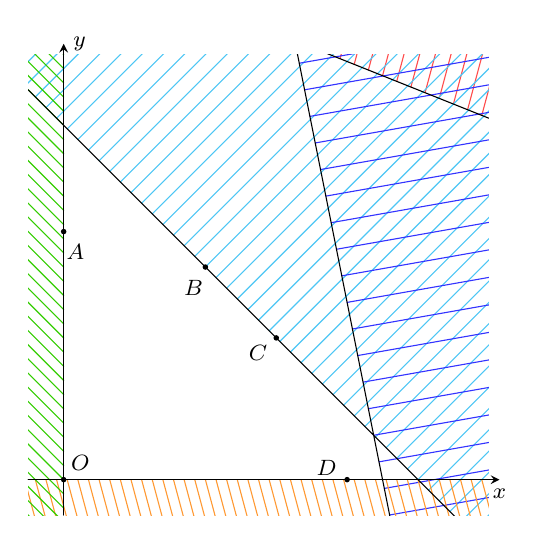
\begin{tikzpicture}[scale=1,font=\footnotesize,line join=round,line cap=round,>=stealth,x=0.45cm,y=0.45cm]
				\tikzset{declare function={f (\x)=15-0.4*(\x); g  (\x)=10-\x; h (\x)=45-5*(\x);}}
				\def\xt{-1} \def\xp{12} 
				\def\yd{-1}  \def\yt{12}
				\begin{scope}
					\clip  (\xt,\yd) rectangle (\xp,\yt);
					\foreach \i in {-3,-2.6,...,\xp}  \draw[red!70!white] (\i,{f (\i)})--++(75:8);
					\foreach \j  in {-2,-1.7,...,\xp} \draw[cyan!70!white] (\j,{g (\j)})--++(45:10);
					\foreach \k in {-1,-0.85,...,\xp} \draw[blue!80!white]  (\k,{h (\k)})--++(10:8);
					\foreach \x  in {-2,-1.7,...,\xp} \draw[orange!80!white] (\x,0)--++(-75:2);
					\foreach  \y in {-2,-1.6,...,\yt} \draw[green!80!red] (0,\y)--++(135:2);
					\draw[domain=\xt:\xp] plot (\x,{f (\x)}) 
						plot (\x,{g (\x)}) 
						plot (\x,{h (\x)}); 
				\end{scope}
				\draw[->] (\xt,0)--(\xp+0.3,0)  node[below]{$x$};
				\draw[->] (0,\yd)--(0,\yt+0.3)  node[right]{$y$};
				\foreach \p/\n/\g in  {(0,0)/O/45,(0,7)/A/-60,(4,6)/B/-120,(6,4)/C/220,(8,0)/D/150} \fill \p node[shift={(\g:3mm)}]{$\n$} circle (1pt);
			\end{tikzpicture}
	\end{center}
	Miền nghiệm của hệ bất phương trình $(1)$ là ngũ giác $OABCD$  với $A(0;7)$; $O(0;0)$; $B(4;6)$, $C(6;4)$, $D(8;0)$. \\
	Vì giá trị lớn nhất của $f(x;y)=70x+90y$ đạt được  tại đỉnh của miền nghiệm.\\
	 Ta có $f(0;0)=0$, $f(0;7)=630$, $f(4;6)=600$, $f(6;4)=580$, $f(8;0)=560$.\\
	Suy ra $f(x;y)$ đạt giá trị lớn nhất tại  $A(0;7)$.\\
	Vậy để đạt số điểm thưởng lớn  nhất đội chơi cần pha chế $7$ lít nước loại B.
	 }
\end{bt}

% nguồn: MaHoaNH_TraLoiNgan_Lop10
\begin{bt}%[0D2V2-3]%[ma:88be5710]
	\immini{Trong mặt phẳng $O x y$, cho tứ giác $A B C D$ có $A(-3; 0)$; $B(0; 2)$; $C(3; 1)$; $D(3;-2)$. Tìm  tất cả các giá trị nguyên của $m$ sao cho điểm $M(m; m-1)$ nằm trong hình tứ giác $A B C D$ kể cả $4$ cạnh.}
	{\begin{tikzpicture}[scale=1,line join=round,line cap=round,>=stealth]
		 \tikzset{every node/.style={scale=1}}
		\def\xmin{-3.5}\def\xmax{4}\def\ymin{-3.5}\def\ymax{4} 
		 \draw[->] (\xmin-0.2,0)--(\xmax+0.2,0) node[below]{$x$};
		\draw[->] (0,\ymin-0.2)--(0,\ymax+0.2) node[right]{$y$}; 
		 \draw (0,0) node[below right]{$O$};
		\clip (\xmin,\ymin) rectangle (\xmax,\ymax); 
		\draw[line width=1.3,fill=black]  (-3,0) circle (1pt) node[above]{$A$}--(0,2) circle (1pt) node[above left]{$B$}--(3,1) circle (1pt) node[above]{$C$}--(3,-2) circle (1pt) node[below]{$D$}--(-3,0)
			(1.3,0.3) circle (1pt) node[right]{$M$}; 
		\foreach \a  in {-2,-1,1,2} \fill (\a,0) circle (1.2pt);
		\foreach \b  in {-3,-2,1,3} \fill (0,\b) circle (1.2pt);
	\end{tikzpicture}
	} 
	 \shortans{3}
	 \loigiai{
		Nhận thấy hình tứ giác $A B C D$ tính cả $4$ cạnh của nó là miền nghiệm của hệ bất phương trình gồm $4$ bất phương trình có miền nghiệm là nửa mặt phẳng  chứa điểm $O(0; 0)$ và lần lượt có các bờ là các đường thẳng $A B$, $B C$, $C D$ và $D A$.\\
		 Phương trình đường thẳng $A B$ là $
		\dfrac{x+3}{0-(-3)}=\dfrac{y-0}{2-0} \Leftrightarrow 2 x-3  y+6=0.$\\
		Bất phương trình có miền nghiệm là là nửa mặt phẳng bờ $A B$ (tính cả bờ $A B$) và chứa điểm  $O$ là $2 x-3 y+6 \geq 0$.\\
		Phương trình đường thẳng $B C\colon \dfrac{x-0}{3-0}=\dfrac{y-2}{1-2} \Leftrightarrow x+3 y-6=0$.\\ Bất phương trình có miền nghiệm là là nửa mặt phẳng bờ $B C$ (tính cả bờ $B C$) và chứa điểm $O$ là $x+3 y-6 \leq 0$.\\ 
		Phương trình đường thẳng  $C D\colon x-3=0$.\\
		Bất phương trình có miền nghiệm là là nửa mặt phẳng bờ $C D$ (tính cả bờ $C D$) và chứa điểm $O$ là $x-3 \leq  0$.\\
		Phương trình đường thẳng $D A\colon \dfrac{x+3}{3-(-3)}=\dfrac{y-0}{-2-0} \Leftrightarrow x+3  y+3=0$.\\
		Bất phương trình  có miền nghiệm là là nửa mặt phẳng bờ $D A$ (tính cả bờ $D A$) và chứa điểm $O$ là $x+3 y+3 \geq 0$.\\
		Hình tứ giác $A B C D$ tính cả $4$ cạnh của nó là miền nghiệm của hệ bất phương trình $$\heva{&2 x-3 y+6 \geq 0 \\& x+3 y-6  \leq 0 \\& x-3 \leq 0 \\& x+3 y+3 \geq 0.}\, \hfill{(1)}$$\\
		Điểm $M(m; m-1)$ nằm trong hình tứ giác $A B C D$  tính cả $4$ cạnh của nó khi và chỉ khi $(m; m-1)$ là một nghiệm của hệ $(1)$, tức là
		 $$
		\heva{& 2 m - 3 ( m - 1) + 6 \geq 0\\& m + 3 ( m - 1) - 6 \leq 0 \\& m - 3 \leq 0 \\& m  + 3 ( m - 1) + 3 \geq 0 }
		\Leftrightarrow \heva{& m \leq 9  \\& m \leq \dfrac{9}{4} \\& m \leq 3 \\&m \geq 0
		} \Leftrightarrow 0 \leq m \leq \dfrac{9}{4}. 
		$$ 
		Vậy các giá trị  của $m$ thỏa mãn là $0 \leq m \leq \dfrac{9}{4}$.\\
		Vậy có $3$ giá trị của $m$ thỏa mãn yêu cầu bài  toán.
	 }
\end{bt}

% nguồn: MaHoaNH_TraLoiNgan_Lop10
\begin{bt}%[0D2V2-3]%[ma:9fd81758]
	Một người bán nước giải khát đang có $25$ gam bột nho và $100$ gam đường để pha chế hai loại nước nho $A$ và $B$. Để pha chế $1$ lít nước nho loại $A$ cần $10$ g đường và $1$g bột nho; để pha chế $1$ lít nước nho loại $B$ cần $10$ gam đường và $4$ gam bột nho. Mỗi lít nước nho loại $A$ khi bán lãi được $30$ nghìn đồng, mỗi lít nước nho loại $B$ khi bán lãi được $40$ nghìn đồng. Hỏi người đó nên pha chế bao nhiêu lít nước nho mỗi loại để  có lợi nhuận cao nhất?
	\shortans{5} 
	\loigiai{ 
		Gọi $x$  và $y$ lần lượt là số lít nước nho loại $A$ và $B$ người đó có thể pha chế.\\
		 Ta có hệ bất phương trình $\heva{&x+4y\le 25\\&x+y\le 10\\&x\ge 0\\&y\ge 0.}$\\
		Miền nghiệm  của hệ bất phương trình là miển tứ giác $OABC$, trong đó $O(0;0)$; $A(10;0);B(5;5);C(0;6{,}25)$.
		\begin{center}
			\begin{tikzpicture}[scale=1.0,font=\footnotesize,line join=round,line cap=round,thick,>=stealth];
					\begin{scope}
						\clip (-1,-1) rectangle (11,7); 
						\fill[pattern=north east lines,opacity=0.5] (-1,-1)--(-1,7)--(11,7)--(11,-1)--cycle; 
						\fill[white] (0,0)--(0,25/4)--(5,5)--(10,0)--cycle; 
						\draw[samples=150,smooth,domain=-1:11] plot (\x,{-0.25*(\x)+25/4}); 
						\draw[samples=150,smooth,domain=-1:11]  plot (\x,{-1*(\x)+10});
					\end{scope}
					\draw[->] (-1,0)--(11,0)  node[below]{$x$};
					\draw[->] (0,-1)--(0,7) node[left]{$y$}; 
					\draw (0,0) node[below left]{$O$}; 
					 \foreach \x in {1,2,3,4,5,6,7,8,9,10}
					 \draw[thin] (\x,1pt)--(\x,-1pt) node [below] {$\x$};
					\foreach  \y in {1,2,3,4,5,6}
					\draw[thin] (1pt,\y)--(-1pt,\y)  node [left] {$\y$};
					\draw (0,25/4) node[below  right]{$C$}
						(5,5) node[below  left]{$B$}
						 (10,0) node[above right]{$A$};
				\end{tikzpicture}
		\end{center}
		Gọi $F$ là số tiền lãi (đơn  vị: nghìn đồng) thu được, ta có $F=30x+40y$.
		\begin{itemize}
			\item Tại $O(0;0):F=30\cdot 0+40\cdot 0=0$. 
			\item Tại $A(10;0):F=30\cdot 10+40\cdot  0=300$.
			 \item Tại $B(5;5):F=30\cdot 5+40\cdot 5=350$.
			 \item Tại $C(0;6{,}25):F=30\cdot 0+40\cdot 6{,}25=250$.
		\end{itemize}
		Ta thấy $F$ đạt  giá trị lớn nhất bằng $350$ tại $B(5;5)$.\\
		Vậy người đó  nên pha chế $5$ lít nước nho mỗi loại đễ có lợi nhuận cao nhất.
	 }
\end{bt}

% nguồn: MaHoaNH_TraLoiNgan_Lop10
\begin{bt}%[0D2V2-3]%[ma:a257cff7]
	Một bãi giữ xe ban đêm dành cho ôtô có diện tích đậu xe là $150$ m$^2$ (không tính lối đi cho xe ra vào). Biết rằng, một xe du lịch cần diện tích $3$ m$^2$ mỗi chiếc và phải trả phí $40$ nghìn đồng mỗi đêm, một xe tải cần diện tích $5$ m$^2$ mỗi chiếc và phải trả phí $50$ nghìn đồng mỗi đêm. Nhân viên quản lí không thể phục  vụ quá $40$ xe một đêm. Doanh thu cao nhất mỗi đêm mà chủ bãi xe thu được là bao nhiêu nghìn đồng.
	\shortans{1750} 
	\loigiai{ 
		\begin{itemize}
			\item Gọi $x$ là số xe du lịch và $y$ là số xe  tải mà chủ bãi xe nên cho đậu một đêm.
			\item Ta có hệ bất phương trình $\heva{&x+y\le  40\\
			 &3x+5y\le 150\\
			&x\ge  0\\
			&y\ge 0}\quad  (I)$
			\item Miền tứ giác $OABC$ là miền  nghiệm của hệ bất phương trình $(I)$, với $O\left(0;0\right)$, $A\left(0;30\right)$, $B\left(25;15\right)$, $C\left(40;0\right)$.
			\begin{center}
				\begin{tikzpicture}[>=stealth,x=1cm,y=1cm,scale=.7]
						\draw[->] (-2,0)--(6,0)  node[below right]{$x$};
						\draw[->] (0,-2)--(0,6) node[left]{$y$}; 
						 \draw (0,0) node[below left]{$O$};
						\path[pattern=horizontal lines]  (-2,6)-|(6,-2)--cycle;
						 \draw (-2,6)--(6,-2);
						 \path[pattern=vertical lines] (-2,4.2)|-(6,6)--(6,-0.6)--cycle;
						\draw (-2,4.2)--(6,-0.6); 
						\path[pattern=crosshatch dots] (-2,-2)  rectangle (0,6);
						 \draw (0,-2)--(0,6);
						\path[pattern=crosshatch] (-2,-2)  rectangle (6,0);
						\draw (-2,0)--(6,0); 
						 \draw[fill=black] (4,0) circle (1pt) node[below][red]{$40$};
						\draw[fill=black] (0,3) circle  (1pt) node[left][red]{$30$};
						\draw[fill=black] (2.5,0) circle (1pt) node[below][red]{$25$}; 
						\draw[fill=black] (0,1.5) circle (1pt) node[left][red]{$15$}; 
						 \draw[dashed] (2.5,0)--(2.5,1.5)--(0,1.5);
					\end{tikzpicture}
			\end{center}
			 \item Số tiền chủ bãi xe thu được $F\left(x;y\right)=40x+50y$ (nghìn đồng)
		\end{itemize}
		Bào toán trở thành tìm giá trị lớn  nhất của $F\left(x;y\right)$ với $F\left(x;y\right)$ thỏa mãn $(I)$.
		\begin{itemize}
			\item Ta có $F\left(0;0\right)=0$, $F\left(0;30\right)=1\,500$; $F\left(25;15\right)=1\,750$; $F\left(40;0\right)=1\,600$. 
		\end{itemize}
		Vậy doanh thu lớn nhất là $1\,750$ nghìn đồng tại điểm có toạ  độ $\left(25;15\right)$.
	} 
\end{bt}

% nguồn: MaHoaNH_TraLoiNgan_Lop10
\begin{bt}%[0D2V2-3]%[ma:28f86fd0]
	Nhân dịp tết Trung thu, xí nghiệp sản xuất bánh muốn sản xuất hai loại bánh: bánh nướng và bánh dẻo. Để sản xuất hai loại bánh này, xí nghiệp cần: đường, bột mì, trứng, mứt bí, lạp xưởng. Xí nghiệp đã nhập về $600\,\mathrm{kg}$ bột mì và $240\,\mathrm{kg}$ đường, các nguyên liệu khác luôn đáp ứng được số lượng mà xí nghiệp cần. Mỗi chiếc bánh nướng cần $120\,\mathrm{g}$ bột mì, $60\,\mathrm{g}$ đường. Mỗi chiếc bánh dẻo cần $160\,\mathrm{g}$ bột mì và $40\,\mathrm{g}$ đường. Theo khảo sát thị trường, lượng bánh dẻo tiêu thụ không vượt quá ba lần lượng bánh nướng và sản phẩm của xí nghiệp sản xuất luôn được tiêu thụ hết. Mỗi chiếc bánh nướng lãi $8\,000$ đồng, mỗi chiếc bánh dẻo lãi $6\,000$ đồng. Để đáp ứng nhu cầu thị trường, đảm bảo lượng bột mì, đường không vượt quá số lượng mà xí nghiệp đã chuẩn bị và vẫn thu được lợi nhuận cao nhất thì xí nghiệp phải sản xuất $m$ chiếc bánh nướng và $n$ chiếc  bánh dẻo, với $m$, $n$ là các số tự nhiên. Tính giá trị $\dfrac{m+2n}{6}$.
	 \shortans{1000}
	 \loigiai{
		 Gọi $x$, $y$ (chiếc) là số lượng bánh nướng, bánh dẻo mà xí nghiệp cần sản xuất. Trong đó $x > 0$, $y > 0$.\\
		 Khối lượng bột mỳ cần dùng là $0{,}12x+0{,}16y \text{ (kg)}$.\\
		Khối lượng  đường cần dùng là $0{,}06x+0{,}04y \text{ (kg)}$.\\
		Ta có $0{,}12x+0{,}16y\le 600$ hay $3x+4y\le  15\,000$;\\
		$0{,}06x+0{,}04y\le 240$  hay $3x+2y\le 12\,000$.\\
		Số tiền lãi thu được là $T=8x+6y$ (nghìn đồng). Bài toán đưa về, tìm $x$, $y$ là nghiệm của hệ bất phương trình $\heva{&3x+4y\le 15\,000\\&3x+2y\le 12\,000\\&y\le 3x\\&x\ge 0\\&y\ge 0}$ (V) để $T=8x+6y$ đạt giá trị lớn nhất.\\ 
		Trước hết, ta biểu diễn miền nghiệm của hệ bất  phương trình (V).
		\begin{center}
			\begin{tikzpicture}[line join=round,line cap=round,>=stealth,thick]
					 \tikzset{every node/.style={scale=0.9}}
					\begin{scope}
						\clip (-1,-1)  rectangle (7,7);
						\fill[pattern=north  west lines] (0,0)--(4,0)--(3,1.5)--(1,3)--cycle;
						\draw  (-1,-3)--(3,9);
						 \draw (-2,9)--(6,-3);
						 \draw (-3,6)--(9,-3);
					\end{scope}
					 \draw[->] (-1.2,0)--(7,0) node[below]{$x$};
					\draw[->]  (0,-1.2)--(0,7) node[left]{$y$};
					\draw (0,0)  node[below left]{$O$};
					\foreach \x  in {1000,3000}
					\draw[thin] (\x/1000,1pt)--(\x/1000,-1pt)  node [below] {$\x$};
					\foreach  \y in {1000,2000,3000}
					 \draw[thin] (1pt,\y/1000)--(-1pt,\y/1000) node [left] {$\y$};
					\draw[dashed,thin] (1,0)--(1,0)--(0,0) 
						 (0,3)--(1,3)--(1,0)
						(0,1.5)--(3,1.5)--(3,0); 
					\fill[black] (4,0) node[above  right]{$A$} circle (1pt)
						(3,1.5) node[right]{$B$}  circle (1pt)
						(1,3)  node[right]{$C$} circle (1pt);
				\end{tikzpicture}
		\end{center}
		Miền nghiệm của hệ bất phương trình là miền tứ giác $OABC$  với $O(0;0)$, $A(4\,000;0)$, $B(3\,000;1\,500)$, $C(1\,000;3\,000)$.\\
		Tính giá trị của $T$ tại các cặp số $(x;y)$ là toạ  độ các đỉnh trên rồi so sánh các giá trị đó, ta được $T$ đạt giá trị lớn nhất bằng $33\,000$ (nghìn đồng) hay $33$ triệu đồng tại $x=3\,000$; $y=1\,500$.\\
		Vậy để đạt được tiền lãi cao nhất, xí nghiệp nên  sản xuất $3\,000$ chiếc bánh nướng và $1\,500$ chiếc bánh dẻo.\\
	Khi đó  $\dfrac{m+2n}{6}=\dfrac{3\,000+2\cdot 1\,500}{6}=1\,000$.}
\end{bt}

% nguồn: MaHoaNH_TraLoiNgan_Lop10
\begin{bt}%[0D2V2-3]%[ma:9022233b]
	Mỗi tuần, một tổ sản xuất được nhà máy cung cấp tối đa $22$ kg nguyên liệu $M$ và $30$ kg nguyên liệu $N$ để sản xuất $10$ sản phẩm gồm các loại $A$, $B$ và $C$. Biết rằng, để sản xuất một sản phẩm loại $A$ cần $3$ kg  nguyên liệu $M$ và 1 kg nguyên liệu $N$; sản xuất một sản phẩm loại $B$ cần 1 kg nguyên liệu $M$ và 3 kg nguyên liệu $N$; sản xuất một sản phẩm loại $C$ cần $2$ kg nguyên liệu $M$ và $4$ kg nguyên liệu $N$. Tiền công sản xuất mỗi sản phẩm loại $A,B,C$ lần lượt là $1{,}2$ triệu đồng, $1{,}3$ triệu đồng và $1{,}5$ triệu đồng. Gọi $x$, $y$, $z$ lần lượt là số sản phẩm loại $A$, $B$, $C$ sản xuất mỗi tuần để số tiền công nhận được là lớn nhất. Tính $T=x+y+z$?
	 \shortans{10}
	\loigiai{ 
		Gọi $x$, $y$ lấn lượt là số sản phẩm loại $A,B$ sản xuất mỗi tuần, thì số sản phẩm loại $C$ sản xuất mỗi tuần là $z=10-x-y$.\\ 
		Khi đó $0\le  x\le 10,0\le y\le 10,0\le x+y\le 10$.\\
		Số lượng nguyên liệu $M$  cần sử dụng $3x+y+2(10-x-y)=x-y+20$ kg.\\
		 Số lượng nguyên liệu $N$ cần sử dụng $x+3y+4(10-x-y)=-3x-y+40$ kg.\\
		 Từ giả thiết bài toán ta có $x-y+20\le 22\Leftrightarrow x-y\le 2$ và $-3x-y+40\le 30\Leftrightarrow 3x+y\ge 10$.\\
		Từ đó  ta thu được hệ bất phương trình $\heva{&0\le x\le 10\\&0\le y\le 10\\&0\le x+y\le 10\quad (*)\\&x-y\le 2\\&3x+y\ge 10}$.\\
		Tiền công nhận được hàng  tuần là
		$$F(x;y)=1{,}2x+1{,}3y+1{,}5(10-x-y)=15-0{,}3x-0{,}2y \text{  (triệu đồng)}.$$
		Ta cần tìm  giá trị lớn nhất của $F(x;y)$ khi $(x;y)$ thỏa mãn hệ bất phương trình.\\
		Ta có miền nghiệm của  hệ bất phương trình $(*)$
		\begin{center}
			\begin{tikzpicture}[scale=1.0,font=\footnotesize,line join=round,line cap=round,thick,>=stealth];
					\begin{scope}
						\clip (-1,-1) rectangle (11,12); 
						\fill[pattern=north east  lines,opacity=0.5] (-1,-1)--(-1,12)--(11,12)--(11,-1)--cycle;
						\fill[white] (0,10)--(3,1)--(6,4)--cycle; 
						\draw  (-1,10)--(11,10)
						 (10,-1)--(10,12);
						\draw[samples=150,smooth,domain=-1:11] plot (\x,{1*(\x)-2}); 
						 \draw[samples=150,smooth,domain=-1:11] plot (\x,{-1*(\x)});
						\draw[samples=150,smooth,domain=-1:11] plot (\x,{-1*(\x)+10}); 
						\draw[samples=150,smooth,domain=-1:11]  plot (\x,{-3*(\x)+10});
					\end{scope}
					\draw[->] (-1,0)--(11,0)  node[below]{$x$};
					\draw[->]  (0,-1)--(0,12) node[left]{$y$};
					\draw (0,0) node[below left]{$O$}; 
					 \foreach \x in {1,2,3,4,5,6,7,8,9,10}
					 \draw[thin] (\x,1pt)--(\x,-1pt) node [below] {$\x$};
					\foreach \y in  {1,2,3,4,5,6,7,8,9,10}
					 \draw[thin] (1pt,\y)--(-1pt,\y) node [left] {$\y$};
					\draw (3,1) node[above]{$N$} 
						 (6,4) node[left]{$O$}
						 (0,10) node[above right]{$M$};
				\end{tikzpicture}
		\end{center}
		Ta có tọa độ các đỉnh  $M(0;10),N(3;1),P(6;4)$.\\
		Suy ra $F(0;10)=13$; $F(3;1)=13{,}9$; $F(6;4)=12{,}4$. 
		So sánh và kết  luận đúng số sản phẩm $A$ cần sản xuất là $3$, số sản phẩm $B$ là $1$ và số sản phẩm $C$ là $6$.\\
		Vậy $T=x+y+z=10$. 
	} 
\end{bt}

% nguồn: MaHoaNH_TraLoiNgan_Lop10
\begin{bt}%[0D2V2-3]%[ma:36a24dd5]
	Tháng 10/1999, mưa lớn kéo dài tại miền Trung đã khiến mực nước các sông lên đến mức kỷ lục, nhất là tại sông Hương. Theo Wikipedia, lúc đó, lượng mưa trong một ngày ở thành phố Huế lên đến $1\,384$ mm. Sau đó, đỉnh lũ ở sông Hương đã lên tới mức  kỷ lục, cao nhất trong vòng 100 năm (tính đến năm 1999). Một khách sạn ở thành phố Huế bị nước lụt tràn vào, cần di chuyển cùng một lúc 80 hành khách và $60$ vali hành lý. Lúc này chỉ huy động được $10$ chiếc ghe lớn và $12$ chiếc ghe nhỏ. Một chiếc ghe lớn chỉ có thể chở 10 hành khách và $9$ vali hành lý. Một chiếc ghe nhỏ chỉ có thể chở 8 hành khách và 6 vali hành lý. Giá một chuyến ghe lớn là $300$ (ngàn đồng) và giá một chuyến ghe nhỏ là $250$ (ngàn đồng). Hỏi chủ khách sạn cần thuê bao nhiêu chiếc ghe mỗi loại để chi phí thấp nhất?
	\shortans{8} 
	\loigiai{ 
		Gọi $x; y$ lần lượt là số ghe  lớn và số ghe nhỏ được chủ khách sạn thuê.
		Ta có hệ bất phương  trình
		$$\heva{& 0 \leq x \leq 1 0  \\
		& 0 \leq y \leq 1  2 \\
		&1 0 x + 8  y \geq 8 0 \\
		&9 x + 6 y \geq 6  0 }
		\Leftrightarrow\heva{ 
		&0  \leq x \leq 10 \\
		& 0 \leq y \leq 12  \\
		& 5 x+4 y \geq 40  \\
		& 3 x+2 y  \geq 20.}$$
		Chi phí chủ khách sạn phải trả thuê  ghe là $F(x; y)=300 \mathrm{x}+250 y$ (ngàn đồng).
		Ta cần tìm  giá trị nhỏ nhất của $F(x; y)$ với $(x; y)$ thỏa mãn hệ bất phương trình $(I)$.
		\begin{center}
			\begin{tikzpicture}[scale=0.4,>=stealth,line join=round,line cap=round,font=\footnotesize,every node/.style={scale=0.8},declare function={
						f  (\x)=10-5/4*(\x);
						g (\x)=10-3/2*(\x); 
						 },x=2 cm,y=2 cm]
					\begin{scope}
						\clip (-1,-1) rectangle  (13,13.5);
						\foreach \x\y\i in{10/0/A,10/12/B,0/12/C,0/10/D,8/0/E} 
						\path (\x,\y)  coordinate (\i);
						\fill[gray] (A)--(B)--(C)--(D)--(E)--cycle; 
						\draw[thick,samples=150,smooth,domain=-2:15] plot (\x,{f (\x)}); 
						 \draw[thick,samples=150,smooth,domain=-2:15] plot (\x,{g (\x)});
						\draw[thick] (-1,12)--(13,12) 
						 (10,-1)--(10,13);
					\end{scope}
					 \draw[->] (-2,0)--(11,0) node[above]{$x$};
					\draw[->] (0,-1)--(0,13) node[left]{$y$}; 
					\fill (0,0) circle (1pt) node[below  left]{$O$}
						 (10,0) circle (1pt) node[above right]{$10$}
						(8,0)  circle (1pt) node[below]{$8$}
						(20/3,0) circle  (1pt) node[below]{$\dfrac{20}{8}$}
						 (0,10) circle (1pt) node[left]{$10$}
						(0,12) circle (1pt) node[above right]{$12$}; 
					 \foreach \i\g in {A/-50,B/50,C/120,D/-20,E/40}
					\fill (\i) circle  (1pt)+(\g:.4) node[scale=.8]{$\i$};
				\end{tikzpicture}
		\end{center}
		Miền nghiệm của hệ bất phương trình trên là đa giác  $A B C D E$ với tọa độ các đỉnh
		 $$
		A(10; 0),  B(10; 12), C(0; 12), D(0; 10), E(8; 0) \text {. }
		$$ 
		Ta  có
		$$ 
		\begin{aligned}
			& F(10; 0)=3000  \\
			 & F(10; 12)=6000 \\
			&  F(0; 12)=3000 \\
			& F(0; 10)=2500  \\
			& F(8;  0)=2400
		\end{aligned}
		$$ 
		Vậy chủ khách sạn  phải thuê $8$ ghe lớn chở khách với chi phí thấp nhất là $2\,400\,000$ đồng.
	} 
\end{bt}


%%%%%%%%%%%%%%%% TỰ LUẬN %%%%%%%%%%%%%%%%

% nguồn: MaHoaNH_TuLuan_Lop10
\begin{bt}%[0D2V2-3]%[ma:6f3281c7]
	Bạn An kinh doanh hai mặt hàng Handmade là vòng tay và vòng đeo cổ. Mỗi vòng tay  làm trong $4$ giờ, bán được $40$ nghìn đồng. Mỗi vòng đeo cổ làm trong $6$ giờ, bán được $80$ nghìn đồng. Mỗi tuần bạn An bán được không quá $15$ vòng tay và $4$ vòng đeo cổ. Tính số giờ tối thiểu trong tuần An cần dùng để bán được ít nhất $400$ nghìn đồng?
	\loigiai{ 
		Gọi $x,y\in \mathbb{N}$ là số vòng tay  và vòng đeo cổ trong tuần An làm được.\\
		Theo giả thiết ta có 
		$\heva{&{40x+80y\ge 400} \\&{0\le x\le 15} \\ 
		&{0\le y\le 4.}}$ \quad $(1)$\\ 
		Bài toán trở thành tìm nghiệm $\left(x,y\right)$ để $L=4x+6y$  nhỏ nhất.\\
		Miền nghiệm của hệ bất phương trình $(1)$ là tam giác $ABC$ với $A(0;50)$,  $B(10;0)$, $C(2;4)$ kể cả miền trong tam giác đó.\\
		Tính giá trị của biểu thức $L=4x+6y$ tại tất cả các đỉnh của  tam giác $ABC$ ta thấy $L$ nhỏ nhất khi $x=2$, $y=4$.\\
		 Vậy số giờ tối thiểu trong tuần An cần dùng là $L=4\cdot2+6\cdot4=32$ giờ.
	 }
\end{bt}

% nguồn: MaHoaNH_TuLuan_Lop10
\begin{bt}%[0D2V2-3]%[ma:b1701a9f]
	Để chế biến một hộp thực phẩm X cần $0{,}2\,\mathrm{kg}$ cà chua và $0{,}1\,\mathrm{kg}$ thịt; một hộp thực phẩm Y cần $0{,}2\,\mathrm{kg}$ cà chua và $0{,}3\,\mathrm{kg}$ thịt. Lợi nhuận thu được từ một hộp  thực phẩm X và một hộp thực phẩm Y lần lượt là $4$ (nghìn đồng) và $5$ (nghìn đồng). Chị Thuỳ mua nhiều nhất $2\,\mathrm{kg}$ cà chua và $2\,\mathrm{kg}$ thịt để chế biến các hộp thực phẩm X và Y. Với lượng nguyên liệu như trên, lợi nhuận lớn nhất chị Thuỳ có thể thu được là bao nhiêu nghìn đồng?
	 \loigiai{
		Gọi $x$ và $y$ lần lượt là số hộp thực phẩm X và Y cần  chế biến.\\
		Khi đó lợi nhuận  thu được là $F(x;y)=4x+5y$.\\
		Từ giả  thiết ta có hệ bất phương trình sau: $\heva{&0{,}1x+0{,}3y\le 2\\&0{,}2x+0{,}2y\le 2\\&x\ge 0\\&y\ge 0.}$\\
		 Miền nghiệm của hệ bất phương trình là miền tứ giác $OACB$ với $A\left(0;\dfrac{20}{3}\right)$, $C(5;5)$, $B(10;0)$, $O(0;0)$.
		\begin{center}
			\begin{tikzpicture}[line join=round,line cap=round,>=stealth,thick]
					\tikzset{every node/.style={scale=0.9}} 
					\begin{scope}
						\clip (-1,-1)  rectangle (6,6);
						\fill[pattern=north east  lines]
						 (0,0)--(5,0)--(2.5,2.5)--(0,10/3)--cycle;
						\draw (-1,6)--(6,-1); 
						\draw  (-2,4)--(13,-1);
					\end{scope}
					\draw[->] (-1,0)--(7,0) node[below]{$x$}; 
					\draw[->]  (0,-1)--(0,6) node[left]{$y$};
					\draw (0,0) node[below left]{$O$}; 
					\fill[black] (5,0) node[above]{$C$}circle  (1pt)
						 (2.5,2.5) node[above right]{$B$}circle (1pt)
						 (0,10/3) node[below left]{$A$}circle (1pt);
				\end{tikzpicture}
		\end{center}
		Ta có $F\left(0;\dfrac{20}{3}\right)=\dfrac{100}{3}$, $F(5;5)=45$, $F(10;0)=40$, $F(0;0)=0$.\\ 
		Giá trị lớn nhất của $F(x;y)=45$ (nghìn đồng) tại  $(5;5)$.\\
	Vậy lợi nhuận lớn nhất chị Thuỳ có  thể thu được là $45$ nghìn đồng khi $x=y=5$.}
\end{bt}

% nguồn: MaHoaNH_TuLuan_Lop10
\begin{bt}%[0D2V2-3]%[ma:eb934ac9]
	Một xưởng cơ khí có hai công nhân là Chiến và Bình. Xưởng sản xuất loại sản phẩm $I$ và $II$. Mỗi sản phẩm $I$ bán lãi $500$ nghìn đồng, mỗi sản phẩm $II$ bán lãi $400$ nghìn đồng. Để sản xuất được một sản phẩm $I$ thì Chiến phải làm việc trong $3$ giờ, Bình phải làm việc trong $1$ giờ. Để sản xuất được một sản phẩm $II$ thì Chiến phải làm việc trong $2$ giờ, Bình phải làm việc trong $6$ giờ. Một người không thể làm được đồng thời hai sản phẩm. Biết rằng trong một tháng Chiến không thể làm việc quá $180$ giờ và Bình không thể làm việc  quá $220$ giờ. Tính số tiền lãi lớn nhất trong một tháng của xưởng.
	\loigiai{ 
		Gọi $x$, $y$  lần lượt là số sản phẩm loại $I$ và loại $II$ được sản xuất ra.\\
		 Điều kiện $x$, $y$ nguyên dương. Ta có hệ bất phương trình sau:
		$\heva{&3x+2y\le 180  \\&x+6y\le 220 \\
		&x > 0 \\&y >  0.}$\\
		Miền  nghiệm của hệ trên là
		\begin{center}
			\begin{tikzpicture}[scale=.4,font=\footnotesize,line join=round,line cap=round,>=stealth]
					\def\xmin{-1.5}\def\xmax{24}\def\ymin{-1}\def\ymax{11} 
					\draw[->] (\xmin,0)--(\xmax,0) node[above]{$x$}; 
					\draw[->] (0,\ymin)--(0,\ymax) node[right]{$y$}; 
					\clip (\xmin,\ymin) rectangle (\xmax,\ymax); 
					\draw[smooth,samples=200,domain=\xmin:\xmax] plot  (\x,{(-1.5)*(\x)+(18/2)});
					 \draw[smooth,samples=200,domain=\xmin:\xmax] plot (\x,{(-1/6)*(\x)+(22/6)});
					\draw (0,9)  node[left]{$90$}; \fill (0,9) circle (1pt);
					\coordinate [label= below:  $A$](A) at (6,0);
					\coordinate [label= above right:  $B$](B) at (4,3);
					\coordinate [label= below left: $C$](C) at  (0,22/6);
					\fill (0,0) circle (1pt)  node[below left]{$O$};
					\draw[pattern=north east lines,draw=none] (A) --  (B) -- (C)-- (0,0)--cycle;
					\foreach \diem in {A,B,C}\fill (\diem) circle (1pt); 
				\end{tikzpicture}
		\end{center}
		Tiền lãi trong một tháng của  xưởng là $T=0{,}5x+0{,}4y$ (triệu đồng).\\
		Ta thấy $T$ đạt giá trị lớn nhất chỉ  có thể tại các điểm $A$, $B$, $C$.\\
		\begin{itemize}
			\item Vì $C$ có tọa độ không nguyên  nên loại.
			\item Tại $A(60;  0)$ thì $T=30$ triệu đồng.
			\item Tại $B(40; 30)$ thì $T=32$ triệu  đồng.
		\end{itemize}
	Vậy tiền lãi lớn nhất trong một tháng  của xưởng là $32$ triệu đồng.}
\end{bt}

% nguồn: MaHoaNH_TuLuan_Lop10
\begin{bt}%[0D2V2-3]%[ma:74a57f96]
	Một hộ nông dân định trồng  dứa và củ đậu trên diện tích $8$ ha. Trên diện tích mỗi ha, nếu trồng dứa thì cần $20$ công và thu $3$ triệu đồng, nếu trồng củ đậu thì cần $30$ công và thu $4$ triệu đồng. Hỏi cần trồng mỗi loại cây trên với diện tích là bao nhiêu ha để thu được nhiều tiền nhất, biết rằng tổng số công không quá $180$.
	 \loigiai{
		Gọi $x$, $y$ lần lượt là số ha trồng dứa và củ  đậu.\\
		Ta có $0\le x\le 8$; $0\le y\le 8$; $x+y\le 8$;  $20x+30y\le 180\Rightarrow 2x+3y\le 18$.\\
		Số tiền  thu được là $T(x;y)=3x+4y$.\\
		Ta có hệ $\heva{&0\le x\le 8 \\&0\le y\le 8 \\&x+y\le 8 \\&2x+3y\le  18.}$\\
		\begin{center}
			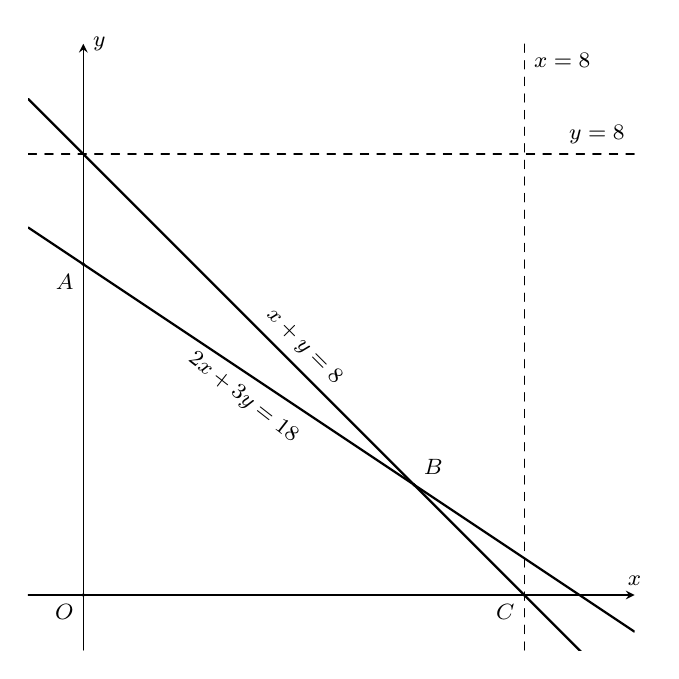
\begin{tikzpicture}[scale=0.7,font=\footnotesize,line join=round,line cap=round,>=stealth]
					 \def\xmin{-1}\def\xmax{10}\def\ymin{-1}\def\ymax{10}
					\draw[->] (\xmin,0)--(\xmax,0) node[above]{$x$}; 
					 \draw[->] (0,\ymin)--(0,\ymax) node[right]{$y$};
					\clip (\xmin,\ymin) rectangle (\xmax,\ymax); 
					\draw[thick,smooth,samples=200,domain=\xmin:\xmax] plot  (\x,{(-1)*(\x)+8});
					\draw[thick,smooth,samples=200,domain=\xmin:\xmax]  plot (\x,{(-2/3)*(\x)+18/3});
					\coordinate  [label= below left: $A$](A) at (0,6);
					\coordinate [label=  above right: $B$](B) at (6,2);
					\coordinate [label= below left: $C$](C)  at (8,0);
					 \fill (0,0) circle (1pt) node[below left]{$O$};
					\draw[dashed]  (8,\ymin)--(8,\ymax) node[below right]{$x=8$}
						(\xmin,8)--(\xmax,8)  node[above left]{$y=8$};
					\draw (5,4) node[rotate=-45,below  left]{$x+y=8$};
					\draw (4.2,3) node[rotate=-38,below  left]{$2x+3y=18$};
					\foreach \diem in {A,B,C}\fill (\diem) circle  (1pt);
				\end{tikzpicture}
		\end{center}
		Miền nghiệm của hệ là miền tứ giác $OABC$ với  $A(0;6)$, $B(6;2)$, $C(0;8)$.\\
		Khi đó $T(x;y)$ đạt cực đại tại một trong  các đỉnh của $OABC$. Khi đó ta có
		\begin{itemize}
			\item $T(0;0)=0$. 
			\item $T(0;6)=24$. 
			 \item $T(6;2)=26$.
			\item  $T(8;0)=24$.
		\end{itemize}
		Vậy cần trồng $6$ ha dứa và $2$  ha củ đậu.
	 }
\end{bt}

% nguồn: MaHoaNH_TuLuan_Lop10
\begin{bt}%[0D2V2-3]%[ma:3435b3f7]
	Một gia đình cần ít nhất $900$ đơn vị protein và $400$ đơn vị lipit trong thức ăn mỗi ngày. Mỗi kilogam thịt bò chứa $800$ đơn vị protein và $200$ đơn vị lipit. Mỗi kilogam thịt lợn chứa $600$ đơn vị protein và $400$ đơn vị lipit. Biết rằng gia đình này chỉ mua nhiều nhất $1{,}6$ kg thịt bò và $1{,}1$ kg thịt lợn. Giá tiền một kg thịt bò là $160$ nghìn đồng, một kg thịt lợn là $110$ nghìn đồng. Gọi $x$, $y$ lần lượt là số kg thịt bò và thịt lợn mà gia đình đó cần mua. Tìm $x$, $y$ để tổng số tiền họ phải trả là ít nhất mà vẫn đảm bảo lượng protein và lipit trong thức ăn? 
	 \loigiai{
		Theo đề bài ta có số tiền gia đình cần trả  là $160x+110y$ với $x$, $y$ thỏa mãn:
		$\heva{&{0\le x\le  1{,}6} \\&{0\le y\le 1{,}1}.}$\\
		Số đơn vị protein gia đình có  là
		$0{,}8x+0{,}6y\ge 0{,}9$ $\Leftrightarrow 8x+6y\ge  9$ $\left(d_1\right)$.\\
		Số đơn vị lipit gia đình  có là $0{,}2x+0{,}4y\ge 0{,}4\Leftrightarrow x+2y\ge 2$ $\left(d_2\right)$.\\
		Tìm $x$, $y$  thỏa mãn hệ bất phương trình $\heva{&0\le x\le 1{,}6\\&0\le y\le 1{,}1\\&8x+6y\ge 9\\&x+2y\ge 2}$ sao cho $T=160x+110y$ nhỏ nhất.
		\begin{center}
			\begin{tikzpicture}[scale=1.5,font=\footnotesize,line join=round,line cap=round,>=stealth]
					 \def\xmin{-1}\def\xmax{4}\def\ymin{-1}\def\ymax{3}
					\draw[->] (\xmin,0)--(\xmax,0)  node[above]{$x$};
					\draw[->] (0,\ymin)--(0,\ymax) node[right]{$y$}; 
					\clip (\xmin,\ymin)  rectangle (\xmax,\ymax);
					\fill[pattern=north east lines] (-1,17/6) -- (\xmin,\ymin)  -- (15/8,-1)-- cycle;
					\draw[smooth,samples=200,domain=\xmin:\xmax] plot  (\x,{(-8/6)*(\x)+(9/6)});
					\fill[pattern=north east lines] (-1,3/2) -- (\xmin,\ymin)  -- (\xmax,-1)-- cycle;
					\draw[smooth,samples=200,domain=\xmin:\xmax] plot (\x,{(-1/2)*(\x)+1}); 
					\coordinate [label=  above right: $A$](A) at (1.6,1.1);
					 \coordinate [label= above right: $B$](B) at (1.6,.2);
					\coordinate [label= above right:  $C$](C) at (.6,.7);
					\coordinate  [label= above right: $D$](D) at (.3,1.1);
					 \fill (0,0) circle (1pt) node[below left]{$O$};
					\foreach  \diem in {A,B,C,D}\fill (\diem) circle (1pt);
					\draw (1.6,\ymin)--(1.6,\ymax) node[below  right]{$x=1{,}6$}
						(\xmin,1.1)--(\xmax,1.1) node[above  left]{$y=1{,}1$};
					\foreach \x in {1,2}\draw  (\x,0.05)--(\x,-0.05) node[below]{$\x$};
					 \foreach \y in {1}\draw (0.05,\y)--(-0.05,\y) node[left]{$\y$};
				\end{tikzpicture}
		\end{center}
		Vẽ hệ trục tọa độ ta tìm được tọa độ các điểm $A(1{,}6; 1{,}1)$; $B(1{,}6; 0{,}2)$; $C(0{,}6; 0{,}7)$;  $D(0{,}3; 1{,}1)$.\\
		Ta có 
		\begin{itemize}
			\item $T(A)=377$ nghìn. 
			 \item $T(B)=278$ nghìn.
			\item $T(C)=173$  nghìn.
			\item $T(D)=169$ nghìn. 
		\end{itemize}
		Vậy tổng số tiền họ phải trả là ít nhất mà vẫn đảm bảo lượng protein và lipit trong thức ăn thì $x=0{,}6$ và  $y=0{,}7$.
	 }
\end{bt}

% nguồn: MaHoaNH_TuLuan_Lop10
\begin{bt}%[0D2V2-3]%[ma:4f8a9b91]
	Một cửa hàng có kế hoạch nhập về hai loại máy tính $A$ và $B$, giá mỗi chiếc lần lượt là $12$ triệu đồng và $20$ triệu đồng với số vốn ban đầu không vượt quá $3{,}6$ tỉ đồng. Loại máy A mang lại lợi nhuận $2$ triệu đồng cho mỗi máy bán được và loại máy B mang lại lợi nhuận là $3$ triệu đồng mỗi máy bán được. Cửa hàng ước tính rằng tổng nhu cầu hàng tháng sẽ không vượt quá $240$ máy. Tìm số lượng máy mỗi loại  mà cửa hàng cần nhập về trong tháng để lợi nhuận thu được là lớn nhất.
	 \loigiai{
		Giả sử trong một tháng cửa hàng  cần nhập số máy tính $A$ là $x$ và số máy tính $B$ là $y$.\\
		Điều kiện: $x\ge  0$; $y\ge 0$.\\
		Do tổng nhu cầu hàng tháng không vượt quá $240$ máy  nên $x+y\le 240$.\\
		Do  số vốn ban đầu không vượt quá $3{,}6$ tỉ đồng nên $12x+20y\le 3600\Leftrightarrow 3x+5y\le 900$.\\
		Do đó, ta  có hệ bất phương trình bậc nhất hai ẩn:
		$$\heva{&x\ge 0\\&y\ge 0\\&x+y\le  240\\&3x+5y\le 900}\quad (I)$$
		Lợi nhuận thu được khi bán $x$ máy tính loại $A$ và $y$ máy tính  loại $B$ là $F(x;y)=2x+3y$ và $F(x;y)=2x+3y$ (triệu đồng).\\
		Ta cần tìm giá trị lớn nhất của  biểu thức $F(x; y)=2x+3y$ với $(x; y)$ thoả mãn hệ bất phương trình (I).\\
		Biểu  diễn miền nghiệm của hệ bất phương trình (I)
		\begin{center}
			\begin{tikzpicture}[scale=1.0,font=\footnotesize,line join=round,line cap=round,thick,>=stealth];
					\begin{scope}
						 \clip (-1,-1) rectangle (11,9);
						\fill[pattern=north east lines,opacity=0.5] (-1,-1)--(-1,9)--(11,9)--(11,-1)--cycle; 
						\fill[white] (0,0)--(0,6)--(5,3)--(8,0)--cycle; 
						\draw[samples=150,smooth,domain=-1:11] plot (\x,{-1*(\x)+8}); 
						\draw[samples=150,smooth,domain=-1:11]  plot (\x,{-3/5*(\x)+6});
					\end{scope}
					\draw[->] (-1,0)--(11,0)  node[below]{$x$};
					 \draw[->] (0,-1)--(0,9) node[left]{$y$};
					\draw  (0,0) node[below left]{$O$};
					\draw (0,6) node[below left]{$A$} 
						(5,3)  node[left]{$B$}
						 (8,0) node[above]{$C$};
					\draw (0,6)  node[above right]{$180$}
						 (8,0) node[below left]{$240$}
						(0,8) node[above  right]{$240$}
						(10,0)  node[below]{$300$};
				\end{tikzpicture}
		\end{center}
		Miền nghiệm của hệ bất phương trình (I) là miền tứ giác $OABC$ với $O(0;0)$, $A(0;180)$, $B(150;90)$, $C(240;0)$ (phần không bị gạch bỏ  trong hình vẽ).\\
		 Ta có bảng giá trị
		\begin{center}
			\begin{tabular}{|c|c|c|c|c|}
				 \hline
				& $O(0;0)$ & $A(0;180)$ & $B(150;90)$  & $C(240;0)$ \\
				\hline 
				$F(x,y)=2x+3y$  & $0$ & $540$ & $570$ & $480$ \\
				 \hline
			\end{tabular}
		\end{center}
		Vậy cần bán $150$ máy tính loại $A$ và $90$ máy tính loại $B$ thì lợi nhuận thu được  là cao nhất.
	} 
\end{bt}

% nguồn: MaHoaNH_TuLuan_Lop10
\begin{bt}%[0D2V2-3]%[ma:5abd35d0]
	Tìm  giá trị lớn nhất biểu thức~ $F\left(x;y\right)=x-y+2024$ với điều kiện $\heva{&2x-y\ge 2\\
	&x-2y\le  2\\
	 &x+y\le 5\\
	&y\ge 0.}\quad(I)$ 
	 \loigiai{
		\begin{itemize}
			\item Vẽ các đường thẳng $d_1\colon 2x-y=2\Leftrightarrow 2x-y-2=0$; $d_2\colon x-2y=2\Leftrightarrow x-2y-2=0$; $d_3\colon x+y=5\Leftrightarrow x+y-5=0$ trên cùng  một hệ trục tọa độ.\\
			Miền nghiệm của  hệ bất phương trình $\left(I\right)$ là miền tứ giác $ABCD$ (phần tô đậm trên hình vẽ).
			\begin{center}
				\begin{tikzpicture}[>=stealth,x=1cm,y=1cm,scale=.7]
						\draw[->]  (-2,0)--(8,0) node[below right]{$x$};
						 \draw[->] (0,-3)--(0,8) node[left]{$y$};
						\draw (0,0) node[below left]{$O$}; 
						\path[pattern=horizontal lines]  (-0.5,-3)-|(-2,8)--(5,8)--cycle;
						\draw (-0.5,-3)--(5,8); 
						 \path[pattern=grid] (-2,-2)|-(8,-3)--(8,3)--cycle;
						\draw (-2,-2)--(8,3); 
						\path[pattern=grid]  (-2,7)|-(8,8)--(8,-3)--cycle;
						\draw (-2,7)--(8,-3); 
						\path[pattern=horizontal lines] (-2,-3) rectangle  (8,0);
						 \draw (-2,0)--(8,0);
						\fill (7/3,8/3) circle (1pt) node[below]{$A$} 
						 (4,1) circle (1pt) node[left]{$B$}
						(2,0)  circle (1pt) node[above]{$C$}
						(1,0) circle (1pt) node[above right]{$D$}; 
					\end{tikzpicture}
			\end{center}
			Trong  đó
			\item $A=d_1 \cap d_3$, tọa độ điểm  $A$ là nghiệm của hệ $\heva{&2x-y=2\\
			&x+y=5} 
			\Leftrightarrow \heva{&x=\dfrac{7}{3}\\ 
			&y=\dfrac{8}{3}} 
			 \Rightarrow A\left(\dfrac{7}{3};\dfrac{8}{3} \right)$.
			\item $B=d_2 \cap d_3$, tọa độ điểm $B$  là nghiệm của hệ $\heva{&x-2y=2\\
			&x+y=5} \Leftrightarrow  \heva{&x=4\\
			 &y=1}
			 \Rightarrow B\left(4;1\right)$.
			 \item $C=d_2 \cap Ox$, tọa độ điểm $C$ là nghiệm của hệ $\heva{&x-2y=2\\
			 &y=0}\Leftrightarrow \heva{&x=2\\
			&y=0} \Rightarrow  C\left(2;0\right)$.
			\item  $D=d_1 \cap Ox$, tọa độ điểm $D$ là nghiệm của hệ $\heva{&2x-y=2\\
			&y=0} \Leftrightarrow  \heva{&x=1\\
			&y=0} \Rightarrow  D\left(1;0\right)$.
		\end{itemize}
		Thay  $x=\dfrac{7}{3};y=\dfrac{8}{3}$ vào $F\left(x;y\right)=x-y+2024$ ta được $F\left(\dfrac{7}{3};\dfrac{8}{3} \right)=\dfrac{6071}{3}$.\\
		Thay $x=4;y=1$ vào $F\left(x;y\right)=x-y+2024$  ta được $F\left(4;1\right)=2027$.\\
		Thay $x=2;y=0$  vào $F\left(x;y\right)=x-y+2024$ ta được $F\left(2;0\right)=2026$.\\
		Thay $x=1;y=0$ vào $F\left(x;y\right)=x-y+2024$  ta được $F\left(1;0\right)=2025$.\\
		Ta có $\dfrac{6071}{3} < 2025< 2026< 2027$.\\ Vậy giá trị lớn nhất  biểu thức $F\left(x;y\right)=x-y+2024$ thỏa mãn điều kiện $\left(I\right)$ là $2027$ tại $\left(4;1\right)$.
	 }
\end{bt}

% nguồn: MaHoaNH_TuLuan_Lop10
\begin{bt}%[0D2B2-3]%[ma:6c9db8de]
	Một biển số xe có mã $71-$C$4$ ở phần trên, phần dưới là một dãy gồm $5$ chữ số chọn  từ các số $0$ đến $9$. Hỏi có thể tạo ra được bao nhiêu biển số xe thỏa điều kiện: Trong dãy $5$ chữ số ở phần dưới, hai chữ số cuối phải là $99$ và ba chữ số đầu phải khác nhau?
	\loigiai{ 
		Gọi dãy $5$ số ở  phần dưới dạng $\overline{a_1a_2a_399}$. Điều kiện: $a_i\neq a_j$ với $i\leq j$ và $i$, $j \in \{1;2;3\}$.\\
		Mỗi cách chọn $a_1$, $a_2$, $a_3$ là một chỉnh hợp $3$ phần tử của $10$. Do  đó, số cách chọn là $\mathrm{A}_{10}^3$.\\
		Vậy số biển số xe thỏa điều kiện đã cho là $\mathrm{A}_{10}^3 =  720$.
	 }
\end{bt}
